\documentclass[../../General.tex]{subfiles}
\begin{document}


\subsection{Módulo de Comunicaciones}

El subsistema de radiocomunicación establece el enlace de intercambio de datos entre el vehículo móvil y el centro de control del parque fotovoltaico, garantizando la transmisión continua de parámetros meteorológicos e indicadores energéticos a lo largo de extensiones de terreno de gran escala mediante una topología descentralizada, mostrada en la Figura \ref{fig:TopologiaRed}.

\begin{figure}[H]
    \captionsetup{justification=raggedright, singlelinecheck=false, labelsep=none}
    \caption[Topología de red con el robot como nodo terminal.]{} 
    \textit{Topología de red con los robots como nodos.} \par\medskip
    \centering
    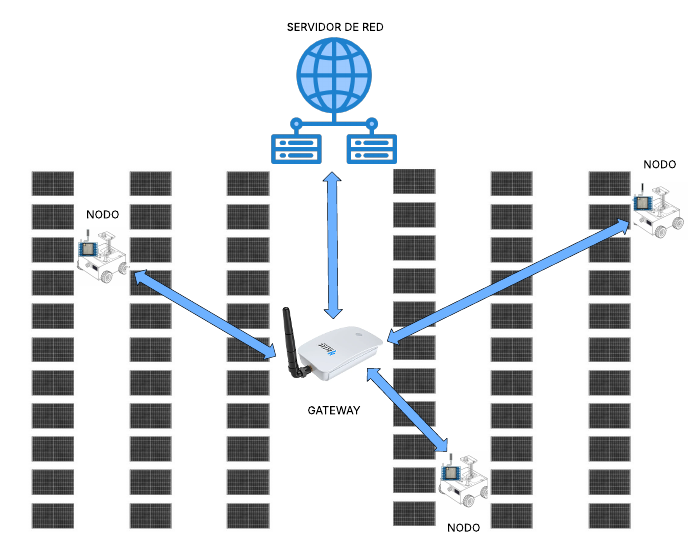
\includegraphics[width=\textwidth]{Recursos/Imagenes/ImagenesDisenoElectronico/TopologiaRedTFC1.png} \par\medskip
    \raggedright
    \footnotesize \textit{Nota.} Elaboración propia.
    \label{fig:TopologiaRed}
\end{figure}

El módulo transceptor de radiofrecuencia corresponde al modelo Ebyte E220-900T30D, sustentado en el circuito integrado Semtech LLCC68. Este dispositivo opera en la banda libre de 915 MHz bajo modulación por espectro ensanchado por chirp, entregando una potencia radiada de hasta un vatio con un consumo continuo de 620 mA y picos de un amperio durante la emisión de ráfagas. Para alcanzar la saturación del amplificador interno sin caídas de tensión, el módulo se alimenta desde la barra limpia de 5.0 V mediante condensadores de tantalio de baja resistencia serie equivalente de cien microfaradios en paralelo con condensadores cerámicos de alta frecuencia.

La interfaz lógica opera de manera directa a 3.3 V comunicándose con los terminales de transmisión y recepción de la computadora monoplaca mediante resistores serie de amortiguación de cincuenta ohmios para mitigar reflexiones de alta frecuencia. La línea de estado de procesamiento incorpora un resistor de polarización a 3.3 V de diez kiloohmios para asegurar un nivel alto durante el arranque del sistema y evitar el ingreso involuntario a la rutina de actualización de firmware, en tanto que dos líneas digitales de la computadora controlan los modos de transmisión transparente, reposo profundo o configuración interna. Los parámetros operativos de la capa física se detallan en la Tabla \ref{tab:capa_fisica_lora}.

\begin{center}
    \footnotesize
    \begin{xltabular}{\textwidth}{|p{3.5cm}|>{\centering\arraybackslash}p{4cm}|>{\raggedright\arraybackslash}X|}
        \caption{Parámetros y configuración de la capa física LoRa para el nodo móvil\label{tab:capa_fisica_lora}} \\
        \hline
        \rowcolor[HTML]{D9E1F2} 
        \textbf{Parámetro de Capa Física} & \textbf{Valor Seleccionado / Ajuste} & \textbf{Justificación Técnica} \\ \hline
        \endfirsthead
        
        \multicolumn{3}{c}%
        {{\bfseries \tablename\ \thetable{} -- Continuación de la página anterior}} \\
        \hline
        \rowcolor[HTML]{D9E1F2} 
        \textbf{Parámetro de Capa Física} & \textbf{Valor Seleccionado / Ajuste} & \textbf{Justificación Técnica} \\ \hline
        \endhead
        
        \hline
        \endfoot
        
        \hline
        \endlastfoot
        
        Banda de Frecuencia & 915 MHz central & Cumplimiento de la banda no licenciada regional en América Latina \\ \hline
        Ancho de Banda & 125 kHz para subida y 500 kHz para bajada & Configuración óptima para maximizar sensibilidad de recepción \\ \hline
        Factor de Dispersión & Factor SF7 & Minimiza el tiempo de ocupación del canal con tasa de 5470 bps \\ \hline
        Tasa de Codificación & Tasa cuatro quintos & Incorpora bits de corrección de errores hacia adelante \\ \hline
        Tamaño de Preámbulo & Ocho símbolos de sincronismo & Garantiza la sincronización de trama entre transceptores \\ \hline
        Modo de Encabezado & Formato explícito & Incluye longitud de carga útil y verificación de redundancia cíclica \\ \hline
        Integridad de Trama & Verificación CRC habilitada & Descarta paquetes corrompidos por interferencia electromagnética \\ \hline
        Polarización de Señal & Estándar para subida e invertida para bajada & Separa lógicamente el tráfico de subida y bajada en la red \\ \hline
    \end{xltabular}
\end{center}

\subsection{Análisis de enlace de radiofrecuencia y balance de pérdidas en espacio libre}

La viabilidad del enlace inalámbrico en las extensiones del parque solar se evalúa mediante el presupuesto de potencia de radiofrecuencia. El transceptor entrega una potencia de transmisión de treinta decibelios milivatio, acoplado a una antena omnidireccional de media onda con ganancia de dos coma quince decibelios isotrópicos montada en el chasis del vehículo. La estación base receptora incorpora una antena con ganancia de tres decibelios isotrópicos y una sensibilidad nominal de recepción de menos ciento veintinueve decibelios milivatio para un ancho de banda de 125 kHz con factor de dispersión nueve. A partir de estos valores, el margen total de ganancia admisible por el hardware se calcula como:

\begin{equation}
M_{\text{enlace}} = P_{\text{tx}} - S_{\text{rx}} = 30.0\text{ dBm} - (-129.0\text{ dBm}) = 159.0\text{ dB}
\end{equation}

Considerando una distancia de enlace en línea de vista de diez kilómetros a la frecuencia central de 915 MHz, las pérdidas de propagación electromagnética en espacio libre se determinan mediante la relación:

\begin{equation}
\begin{split}
\text{FSPL} &= 20\log_{10}(d) + 20\log_{10}(f) - 147.55 \\
&= 20\log_{10}(10000) + 20\log_{10}(915\times 10^6) - 147.55 \approx 111.68\text{ dB}
\end{split}
\end{equation}

Deduciendo las pérdidas por inserción de conectores coaxiales estimadas en medio decibelio e integrando las ganancias de ambas antenas, el margen de desvanecimiento resultante para la comunicación se expresa como:

\begin{equation}
M_{\text{desvanecimiento}} = 159.0\text{ dB} + 2.15\text{ dBi} + 3.00\text{ dBi} - 0.50\text{ dB} - 111.68\text{ dB} \approx 51.97\text{ dB}
\end{equation}

La obtención de un margen superior a cincuenta decibelios garantiza una elevada robustez operativa frente a obstáculos del terreno, atenuación atmosférica por precipitación y dispersiones provocadas por estructuras metálicas de los paneles solares.

\subsection{Dimensionamiento de la trama de transmisión e integración con plataformas supervisoras}

La comunicación inalámbrica transfiere periódicamente los parámetros operativos hacia el centro de control mediante una estructura binaria optimizada de veintiún bytes basada en el estándar Cayenne Low Power Payload, evitando el desperdicio de ancho de banda derivado de formatos en texto plano. La distribución detallada de los campos de datos se expone en la Tabla \ref{tab:payload_mapping}.

\begin{center}
    \footnotesize
    \begin{xltabular}{\textwidth}{|c|>{\centering\arraybackslash}p{2.5cm}|>{\raggedright\arraybackslash}X|c|}
    \caption{Estructura y mapeo de bytes de la trama de telemetría de veintiún bytes\label{tab:payload_mapping}} \\
    \hline
    \rowcolor[HTML]{D9E1F2} 
    \textbf{Bytes} & \textbf{Campo} & \textbf{Descripción y Escala} & \textbf{Tipo de Dato} \\ \hline
    \endfirsthead
    
    \multicolumn{4}{c}%
    {{\bfseries \tablename\ \thetable{} -- Continuación de la página anterior}} \\
    \hline
    \rowcolor[HTML]{D9E1F2} 
    \textbf{Bytes} & \textbf{Campo} & \textbf{Descripción y Escala} & \textbf{Tipo de Dato} \\ \hline
    \endhead
    
    \hline
    \endfoot
    
    \hline
    \endlastfoot
    
    0 & Identificador de Nodo & Código numérico único del robot móvil & Entero sin signo de 8 bits \\ \hline
    1 & Contador de Trama & Secuencia consecutiva de paquete emitido & Entero sin signo de 8 bits \\ \hline
    2 al 3 & Irradiancia Solar & Lectura de radiación en vatios por metro cuadrado & Entero sin signo de 16 bits \\ \hline
    4 al 5 & Temperatura Ambiente & Registro térmico en centésimas de grado & Entero con signo de 16 bits \\ \hline
    6 al 7 & Humedad Relativa & Porcentaje de humedad en centésimas & Entero sin signo de 16 bits \\ \hline
    8 al 9 & Celeridad del Viento & Magnitud de viento en décimas de metro por segundo & Entero sin signo de 16 bits \\ \hline
    10 al 13 & Latitud Geográfica & Coordenada satelital escalada a siete decimales & Entero con signo de 32 bits \\ \hline
    14 al 17 & Longitud Geográfica & Coordenada satelital escalada a siete decimales & Entero con signo de 32 bits \\ \hline
    18 al 19 & Banderas de Estado & Nivel de batería y alertas de seguridad & Entero sin signo de 16 bits \\ \hline
    20 & Verificación de Carga & Suma de redundancia para la capa de aplicación & Entero sin signo de 8 bits \\ \hline
\end{xltabular}
\end{center}

Con un factor de dispersión de $7$ ($SF7$) y un ancho de banda de $125\text{ kHz}$, el tiempo en el aire (\textit{time-on-air}) para transmitir este paquete de $21\text{ bytes}$ es inferior a $50\text{ ms}$, lo que permite actualizaciones continuas sin saturar el canal de radiofrecuencia y facilita la recepción en pasarelas concentradoras conectadas a servidores de supervisión industrial.

\subsection{Receptor satelital multiconstelación y sincronización temporal con respaldo de energía}

La georreferenciación del vehículo y la sincronización horaria de los registros meteorológicos se resuelven mediante el módulo de navegación u-blox SAM-M8Q. Este receptor procesa concurrentemente señales procedentes de las constelaciones GPS, GLONASS y Galileo junto a sistemas de aumento basados en satélites, alcanzando una sensibilidad de navegación de $-165\text{ dBm}$. El circuito incorpora en su cara superior una antena cerámica pasiva de polarización circular derecha de $15\text{ mm}$ de lado, complementada por un amplificador de bajo ruido y un filtro de ondas acústicas superficiales para rechazar emisiones fuera de banda.

El dispositivo se comunica con la computadora de a bordo mediante un enlace serial asíncrono (UART) a $3.3\text{ V}$ en las terminales de transmisión y recepción, ejecutándose en el sistema operativo un servicio en segundo plano encargado de decodificar las sentencias estándar NMEA a una frecuencia de actualización de $1\text{ Hz}$. Para evitar retardos de hasta $30\text{ s}$ en la adquisición de efemérides satelitales al encender el equipo en campo, el módulo integra una microbatería recargable de litio-manganeso de $3\text{ V}$ que mantiene energizados el reloj de tiempo real y la memoria SRAM interna cuando la alimentación principal se interrumpe. Este respaldo permite realizar arranques en caliente con fijación de posición en menos de $2\text{ s}$, asegurando la disponibilidad inmediata de coordenadas espaciales para el inicio de las misiones autónomas.

%%%--------------------------------------------------------------------------------------------%%%
%%%--------------------------------------------------------------------------------------------%%%

\begin{figure}[H]
	% Fuerza la alineación izquierda y quita los ":" después del número
	\captionsetup{justification=raggedright, singlelinecheck=false, labelsep=none}
	
	\caption[.]{}
	
	\textit{.}\par\medskip
	
	\centering
	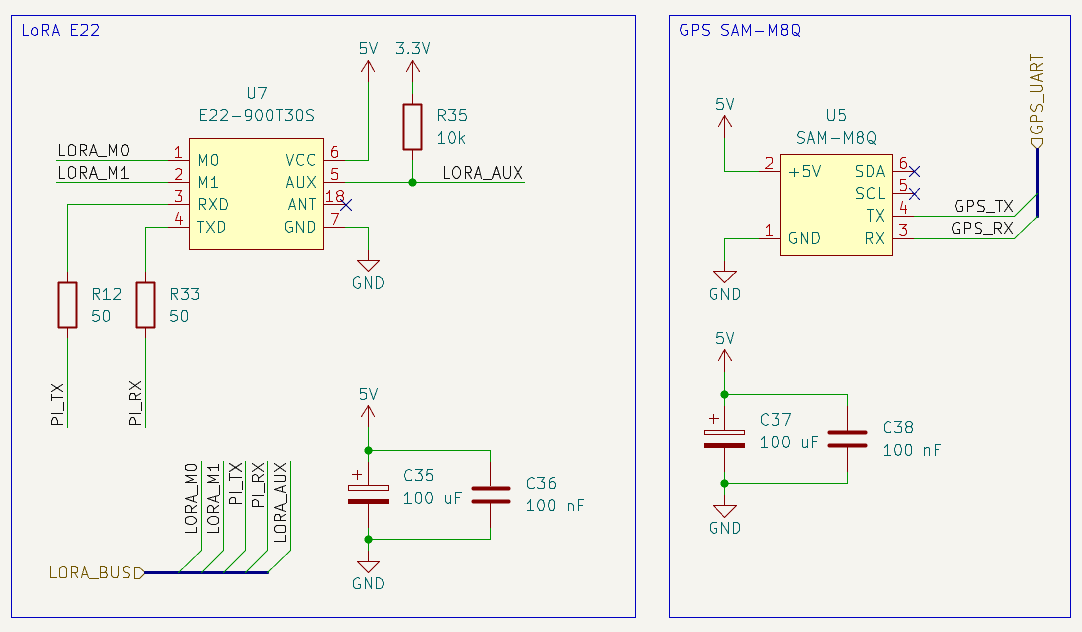
\includegraphics[width=\textwidth]{Recursos/Imagenes/ImagenesDisenoElectronico/LoRaGPS.png} \par\medskip
	
	\raggedright
	\footnotesize \textit{Nota.} Elaboración propia.
	\label{fig:LoRaGPS}
\end{figure}
%%%


\end{document}